\documentclass[tikz,border=5pt]{standalone}
\usepackage{amsmath,amssymb}
\begin{document}
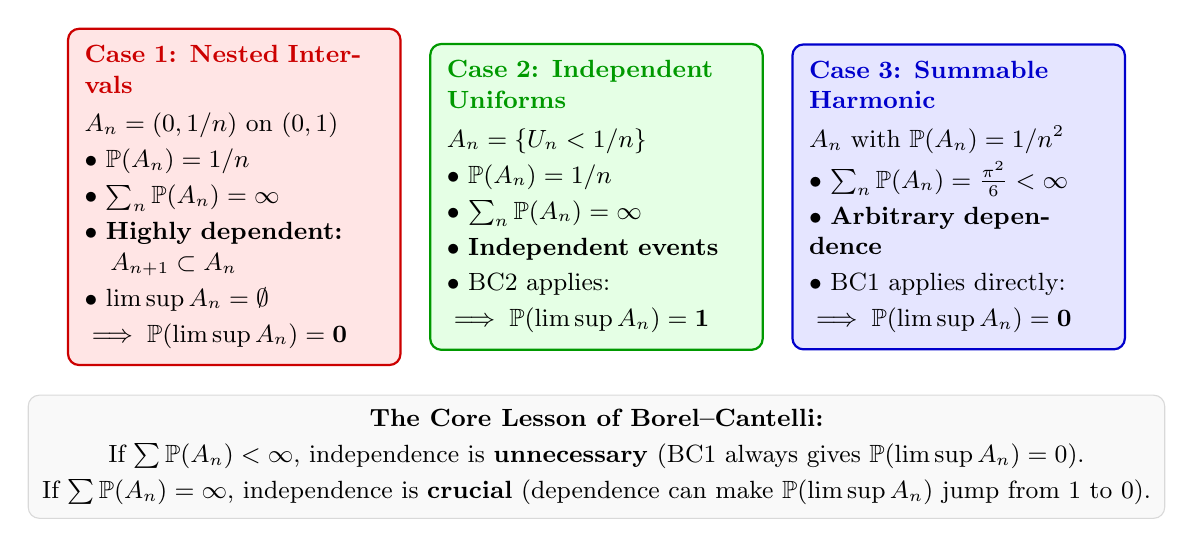
\begin{tikzpicture}[>=latex, font=\small]
  % Case 1
  \begin{scope}[xshift=0cm]
    \node[draw=red!80!black, fill=red!10, rounded corners, thick, text width=3.8cm, inner sep=6pt, align=left] at (0, 0) {
      \textbf{\color{red!80!black}Case 1: Nested Intervals}\\[3pt]
      $A_n = (0, 1/n)$ on $(0,1)$\\[2pt]
      $\bullet$ $\mathbb{P}(A_n) = 1/n$\\[2pt]
      $\bullet$ $\sum_{n} \mathbb{P}(A_n) = \infty$\\[2pt]
      $\bullet$ \textbf{Highly dependent:}\\
      \quad $A_{n+1} \subset A_n$\\[2pt]
      $\bullet$ $\limsup A_n = \emptyset$\\[2pt]
      $\implies \mathbb{P}(\limsup A_n) = \mathbf{0}$
    };
  \end{scope}

  % Case 2
  \begin{scope}[xshift=4.6cm]
    \node[draw=green!60!black, fill=green!10, rounded corners, thick, text width=3.8cm, inner sep=6pt, align=left] at (0, 0) {
      \textbf{\color{green!60!black}Case 2: Independent Uniforms}\\[3pt]
      $A_n = \{U_n < 1/n\}$\\[2pt]
      $\bullet$ $\mathbb{P}(A_n) = 1/n$\\[2pt]
      $\bullet$ $\sum_{n} \mathbb{P}(A_n) = \infty$\\[2pt]
      $\bullet$ \textbf{Independent events}\\[2pt]
      $\bullet$ BC2 applies:\\[2pt]
      $\implies \mathbb{P}(\limsup A_n) = \mathbf{1}$
    };
  \end{scope}

  % Case 3
  \begin{scope}[xshift=9.2cm]
    \node[draw=blue!80!black, fill=blue!10, rounded corners, thick, text width=3.8cm, inner sep=6pt, align=left] at (0, 0) {
      \textbf{\color{blue!80!black}Case 3: Summable Harmonic}\\[3pt]
      $A_n$ with $\mathbb{P}(A_n) = 1/n^2$\\[2pt]
      $\bullet$ $\sum_{n} \mathbb{P}(A_n) = \frac{\pi^2}{6} < \infty$\\[2pt]
      $\bullet$ \textbf{Arbitrary dependence}\\[2pt]
      $\bullet$ BC1 applies directly:\\[2pt]
      $\implies \mathbb{P}(\limsup A_n) = \mathbf{0}$
    };
  \end{scope}

  \node[align=center, fill=gray!5, draw=gray!30, rounded corners, inner sep=5pt] at (4.6, -3.3)
    {\textbf{The Core Lesson of Borel–Cantelli:}\\[2pt]
     If $\sum \mathbb{P}(A_n) < \infty$, independence is \textbf{unnecessary} (BC1 always gives $\mathbb{P}(\limsup A_n) = 0$).\\[2pt]
     If $\sum \mathbb{P}(A_n) = \infty$, independence is \textbf{crucial} (dependence can make $\mathbb{P}(\limsup A_n)$ jump from $1$ to $0$).};
\end{tikzpicture}
\end{document}
